%----------------------------------------------------------------------------
\chapter{Kliens oldal}
\label{chapt:birdmap-frontend}
%----------------------------------------------------------------------------
Ebben a fejezetben bemutatom a kliensoldal architektúráját. Ismertetem a különböző komponensek felépítését.

%----------------------------------------------------------------------------
\section{Architektúra}
%----------------------------------------------------------------------------
Az alkalmazásnak minden oldala egy külön React komponens, mely mindegyikének saját mappája van a főkönyvtár alatt, 
ahol az egyes oldalak által használt szolgáltatások és egyéb komponensek találhatóak.
A közöses használt szolgáltatások és komponensek a common mappába kerültek.

A kliensoldal belépési pontja az \verb+App.js+ fájlban található \verb+App+ komponens.
Itt egy React \verb+Switch+-ben fel van sorolva az összes oldal komponense azok elérési útvonalai szerint.
Ezt szemlélteti a \ref{lst:react-switch}-es lista.
Az a komponens jelenik meg a felületen, amelyiknek \verb+path+ mező értéke megegyezik az URL-ben találhatóval.

\begin{lstlisting}[style=jsx, caption=Az App.js Switch tartalma., label=lst:react-switch]
<Switch>
    <PublicRoute exact path="/login" component={AuthComponent} />
    <AdminRoute exact path="/logs" component={LogsComponent} />
    <DevicesContextProvider>
        <PrivateRoute exact path="/" component={DashboardComponent} />
        <PrivateRoute exact path="/devices/:id?" component={DevicesComponent} />
        <PrivateRoute exact path="/heatmap" component={HeatmapComponent} />
    </DevicesContextProvider>
</Switch>
\end{lstlisting}

Hozzáférés szempontjából három fajta oldalt különböztetünk meg:
\begin{itemize}
    \item \textbf{Publikus oldal}. Az oldal bejelentkezés nélkül is látogatható.
    \item \textbf{Privát oldal}. Az oldal csak bejelentkezés után látogatható.
    \item \textbf{Admin oldal}. Az oldalt csak bejelentkezett admin felhasználók látogathatják.
\end{itemize}

Ezek alapján készítettem két generikus komponenst. Az egyik a \verb+DefaultLayout+ komponens, mely az oldal alapértelmezett elrendezéséért felel.
Paraméterében át lehet adni egy másik megjeleníteni kívánt komponenst, melyet a fejléc alatt jelenít meg.
Mivel minden komponens ebbe az bázis komponensbe van csomagolva, így akárhova navigálunk az oldalon a felület mindig egységes marad.

A másik komponens a \verb+PredicateRoute+, melynek paraméterében meg lehet adni egy feltételt, illetve egy másik komponenst.
Ha a feltétel hamis akkor átírányítja a felhasználót a bejelentkező oldalra, ha igaz akkor megjeleníti a \verb+DefaultLayout+-ba csomagolt komponenst.
Publikus oldalnál a feltétel mindig igaz. 
Privátnál a feltétel a bejelentkezéshez van kötve. 
Az admin oldal feltétele egyrészt szintén a bejelentkezés, másrészt a felhasználó \verb+Admin+ jogolsultsága.
Ezt a folyamatot próbálja szemléltetni a \ref{fig:birdmap-frontend-architecture}-es ábra. 
Legfelül sárgával vannak feltüntetve a hívható végpontok, alattuk a hozzájuk kapcsolt megjelenítendő komponensek, azok alatt pedig a hozzáférést szabályozó komponensek.

\begin{figure}[!ht]
    \centering
    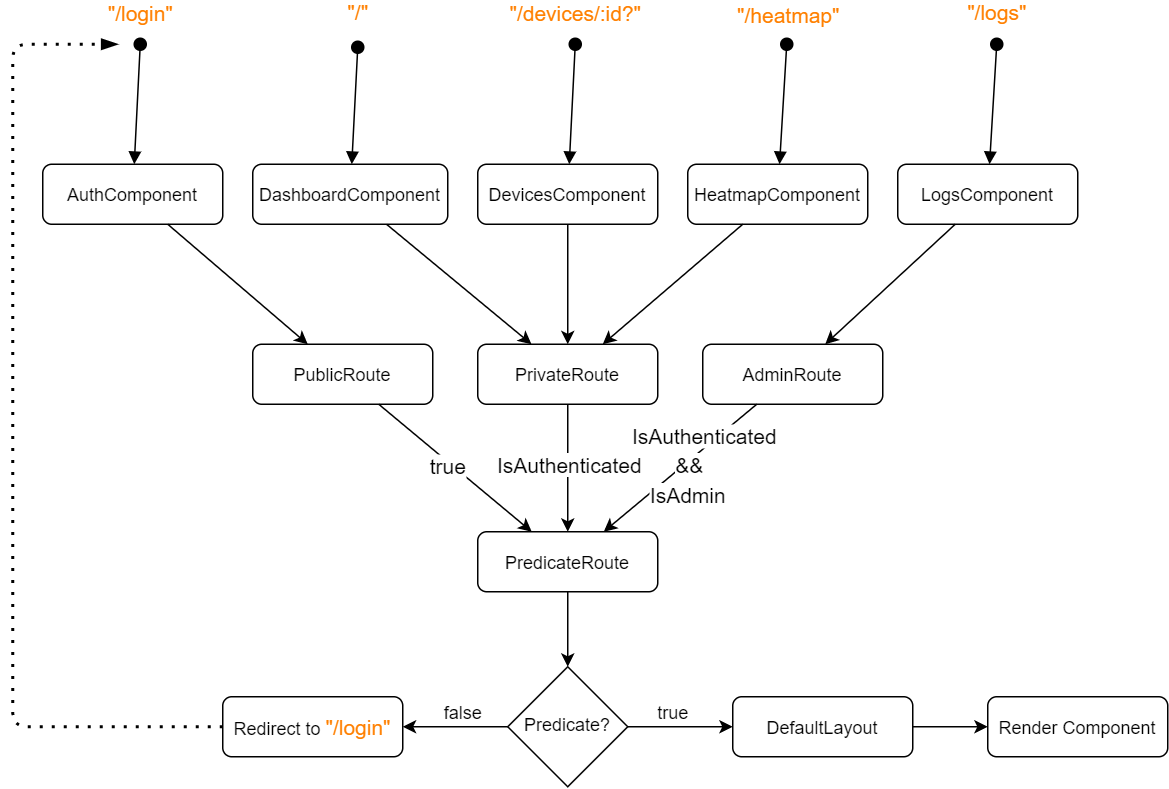
\includegraphics[width=150mm, keepaspectratio]{figures/birdmap-frontend-routes.png}
    \caption{A Birdmap kliensoldalának architektúrája}
    \label{fig:birdmap-frontend-architecture}
\end{figure}

%----------------------------------------------------------------------------
\section{Kommunikáció a szerveroldallal}
%----------------------------------------------------------------------------
A szerveroldallal való kommunikációt rendkívül egyszerűen tudtam implementálni köszönhetően a \ref{subsect:backend-swagger}-as fejezetben bemutatott Swagger oldalnak
és annak, hogy az NSwag Studio-val\cite{nswag-studio} a C\#-on kívül lehet TypeScript\footnotemark klienseket is generálni a leíró fájlból.
Így készültek el a kommponensek kommunikációért felelős szolgáltatásai.

\footnotetext{JavaScript-re épített statikus típusdefiníciókat tartalmazó nyelv. JavaScript és TypeScript együtt is használható.}
%----------------------------------------------------------------------------
\section{Komponensek}
%----------------------------------------------------------------------------
Ebben a szakaszban ismertete az egyes oldalak komponenseit és azok alkomponenseit,
illetve a navigációért felelős fejlécet.
%----------------------------------------------------------------------------
\subsection{Navigáció}
%----------------------------------------------------------------------------
A fejléc két komponensből áll. Az egyik az oldal címe a másik az oldalak linkjeit tartalmazó komponens.
Utóbbit a React \verb+NavLink+ komponenseivel készítettem, melyeknek meg lehet adni, hogy kattintásra hova irányítsa a felhasználót.
Ha a jelenlegi webcím tartalmazza a linknek megadott címet, akkor az aktív státuszba kerül, melyre külön stílus osztályok vonatkoznak.
Ezt használva, az aktív linkeket egy aláhúzással jelölöm. 

\begin{figure}[!ht]
    \centering
    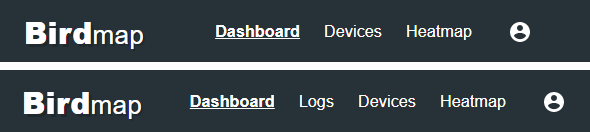
\includegraphics[width=150mm, keepaspectratio]{figures/appbar-user-admin.png}
    \caption{A Birdmap fejléce. Felül a User, alul az Admin felhasználóké}
    \label{fig:birdmap-appbar}
\end{figure}

A fejléc alapértelmezetten része a \verb+DefaultLayout+ komponensnek, így minden oldalon megjelenítésre kerül.

%----------------------------------------------------------------------------
\subsection{Login}
%----------------------------------------------------------------------------
A bejelentkező oldal viszonylag egyszerű. Két szövegdobozt és egy bejelentkező gombot tartalmaz, ahogy az a \ref{fig:birdmap-login}-as ábrán is látszik.

\begin{figure}[!ht]
    \centering
    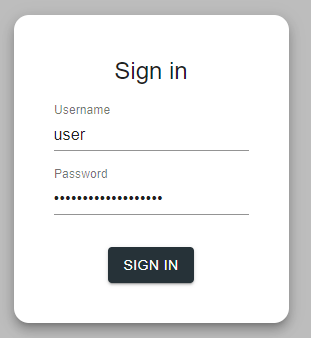
\includegraphics[width=60mm, keepaspectratio]{figures/birdmap-login.png}
    \caption{A Birdmap bejelentkező felülete}
    \label{fig:birdmap-login}
\end{figure}

A generált szerverrel kommunikáló szolgáltatás be van csomagolva egy közösen használt másik szolgáltatásba.
Ennek célja, hogy a bejelentkezés eredményét több komponens is olvashassa, hiszen az alkalmazás felületét alapvetően megkülönbözteti,
egyrészt a bejelentkezés sikeressége, másrészt a bejelentkezett felhasználó jogosultsági köre.

Sikeres bejelentkezés után a szerver elküldi a felhasználó szerepét, illetve a hozzáférési token-t, amelyre a kliens többi szolgáltatásának is szüksége lesz a kommunkációhoz. 
Ezeket az oldal \verb+sessionStorage+-ában\footnotemark tárolom és a becsomagolt szolgáltatáson keresztül elérhetőek.

Kijelentkezni a navigációs fejlécben található profil ikonra való kattintással lehet.

\footnotetext{Webtárhely objektum. Lehetővé teszi a kulcs-érték párok tárolását a böngészőben.}

%----------------------------------------------------------------------------
\subsection{Logs}
%----------------------------------------------------------------------------
Ez az oldal az \verb+Admin+ felhasználó számára lehetővé teszi a szerveren található naplófájlok letöltését \verb+zip+ fájlformátumú archív fájlokban.
Komponense a \ref{fig:birdmap-logs}-es ábrán látható.

\begin{figure}[!ht]
    \centering
    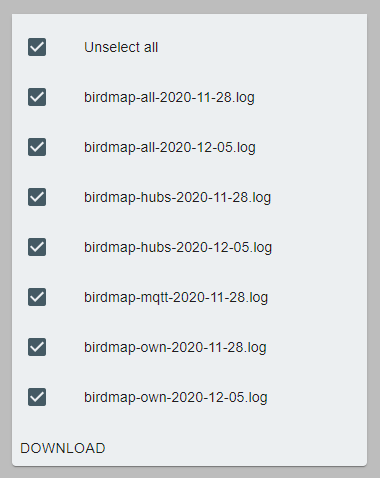
\includegraphics[width=75mm, keepaspectratio]{figures/birdmap-logs.png}
    \caption{A Birdmap naplófájlok letöltésének felülete}
    \label{fig:birdmap-logs}
\end{figure}
%----------------------------------------------------------------------------
\subsection{Eszköz állapot és hangüzenet kezelő szolgáltatás}
%----------------------------------------------------------------------------
A szakasz további komponenseinek van egy közös ismertetője. Mégpedig, hogy mindegyiknek szüksége van a kihelyezett eszközök adataira
és az azok által publikált hangüzenetekből képzett valószínűségre.
A Reactnek van egy beépített komponense \verb+Context+\cite{react-context} néven, mellyel különböző komponensek között lehet adatokat megosztani.
Ezt használva készítettem egy \verb+DevicesContextProvider+ osztályt, melynek feladata a szerver eszköz kontrollerével való kommunikáció a megfelelő szolgáltatáson keresztül,
illetve a SignalR csatornákra való feliratkozás. Ezekből az adatokból egy \verb+DevicesContext+ készül, mely a \verb+Provider+ által átadásra kerül annak minden gyerekének.
A \ref{lst:react-switch}-es listában látható, hogy a \verb+DevicesContextProvider+ szülője a \verb+Dashboard+, \verb+Devices+ és \verb+Heatmap+ komponenseknek.

%----------------------------------------------------------------------------
\subsection{Dashboard}
%----------------------------------------------------------------------------
A Dashboard az alkalmazás kezdő oldala. Itt található meg a külső szolgáltatások állapotát vizsgáló komponens,
illetve a kihelyezett eszközök működési folyamatában áttekintést nyújtó diagrammok mindegyike.

Az oldal megjelenítésekor elindul egy másodpercenként ismétlődő folyamat,
mely a \verb+DevicesContext+-ből kiolvasott értékekből legenerálja a diagrammokon megjelenítendő összes adatot.
Ez azonban az adat mennyiségétől függően akár egy-két másodpercig is eltarthat, ami rendkívül lassúvá és használhatatlanná tenné a felületet.
Ennek elkerülése érdekében az adatfeldolgozó folyamat egyszerre csak egy pár elemet dolgoz fel, mely alfolyamatok között 20 milliszekundum szüneteket iktattam be.
Továbbá hogy a különböző diagrammok animációi is zökkenőmentesek legyenek, azok adatai cserélése között is van 300 milliszekundum szünet.
Így valamivel lasabb az adatfeldolgozás, de a felület használható marad.
%----------------------------------------------------------------------------
\subsubsection{Külső szolgáltatások}
%----------------------------------------------------------------------------
Az alkalmazás használatának szempontjából van néhány olyan külső szolgáltatás, melyek elérhetősége hiányában a rendszer működésképtelen.
Ilyen például a Birdnetes klasztere vagy a szerver MQTT szolgáltatása. 
Ezért készítettem el az \ref{fig:dashboard-services-loaded}-ös ábrán látható információs panelt, ahol a szolgáltatások állapotát lehet látni, hogy a felhasználó tudja miért nem működik esetleg az alkalmazás.
A felület megvalósításhoz a Material UI \verb+Accordion+ elemét használtam, ami lényegében egy lenyíló lista. 
Ennek fejlécében a szolgáltatás neve, elérési útvonala és státusza látható. A lenyíló elemben a szolgáltatástól érkezett válasz van megjelenítve. 

\begin{figure}[!ht]
    \centering
    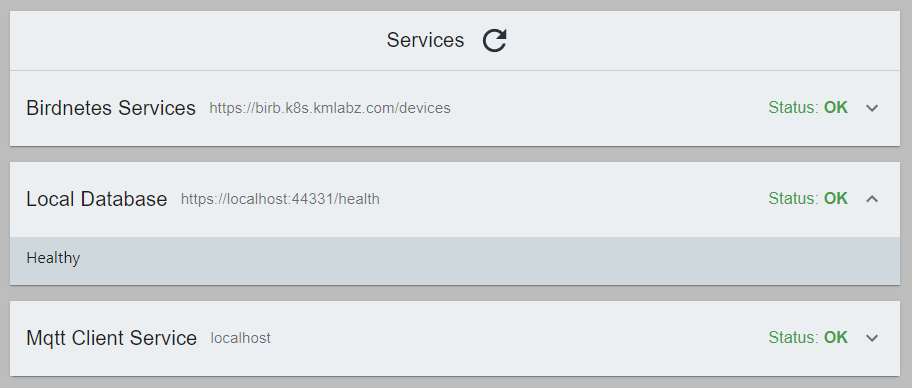
\includegraphics[width=150mm, keepaspectratio]{figures/dashboard-services-loaded.png}
    \caption{Az alkalmazás által használt külső komponensek állapotának megjelenítéséért felelős komponens}
    \label{fig:dashboard-services-loaded}
\end{figure}

Az oldal betöltése vagy a frissítés gomb megnyomása esetén az adatok lekérésre kerülnek a szervertől.
Ez a folyamat akár öt-hat másodpercig is eltarthat, mely közben a felhasználó egy üres listát látna.
Ennek elkerülésére használom a Material UI \verb+Skeleton+ komponensét, 
mely egy megadható méretű töltő csíkkal helyettesíti az \verb+Accordion+-ban található elemeket a \ref{fig:dashboard-services-loading}-os ábrán látható módon.
Azért célszerű ennek a használata, mert így a felhasználónak több információja van arról, hogy a felületen milyen adatok és hol fognak megjelenni.
A felhasználói élmény maximalizálása érdekében a frissítés előtt lekérdezem a szervertől, hogy hány darab szolgáltatás található az adatbázisban 
és annyi darab töltőcsíkos \verb+Accordion+-t jelenítek meg. 

\begin{figure}[!ht]
    \centering
    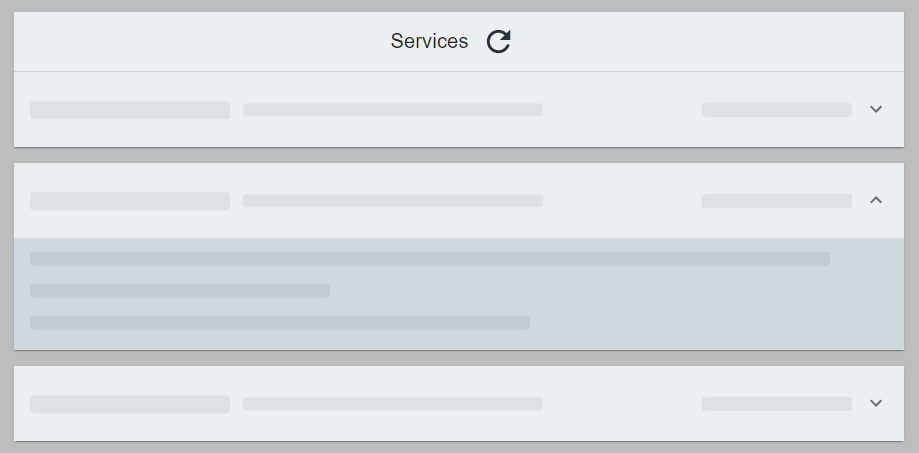
\includegraphics[width=150mm, keepaspectratio]{figures/dashboard-services-loading.png}
    \caption{A Skeletonok alkalmazása a külső szolgáltatások állapotának betöltése közben.}
    \label{fig:dashboard-services-loading}
\end{figure}

%----------------------------------------------------------------------------
\subsubsection{Eszközök és szenzorok állapota}
%----------------------------------------------------------------------------
Ennek a komponensnek a szerepe, hogy áttekintést nyújtson az eszközök és szenzorok állapotáról.
Úgy gondoltam, hogy erre a legcélravezetőbb eszköz a \ref{fig:dashboard-donut}-es ábrán is látható Apexcharts fánk diagrammja.
Látható, hogy hány darab eszköz és szenzor van bekapcsolt, kikapcsolt, illetve hibás állapotban.
Az állapotok változása esetén a \verb+DevicesContextProvider+-nek köszönhetően az adatok automatikusan frissülnek.
\begin{figure}[!ht]
    \centering
    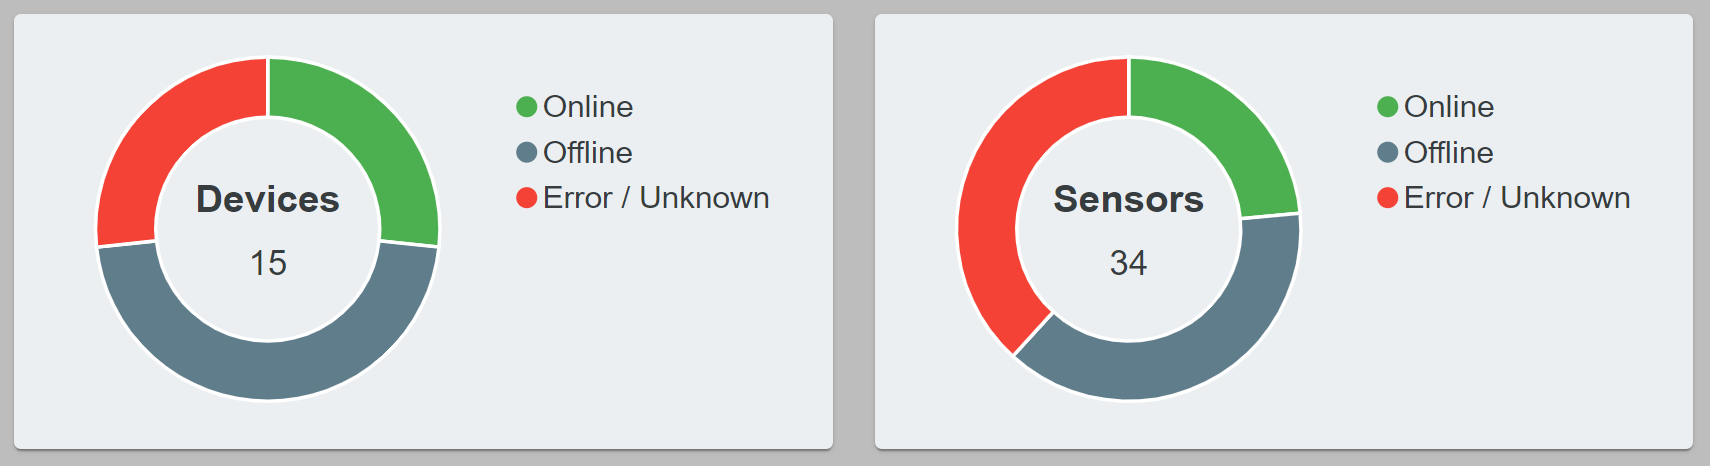
\includegraphics[width=150mm, keepaspectratio]{figures/dashboard-donut-devices.png}
    \caption{A Dashboard eszköz- és szenzor állapotok diagrammja}
    \label{fig:dashboard-donut}
\end{figure}
%----------------------------------------------------------------------------
\subsubsection{Hőtérkép diagrammok}
%----------------------------------------------------------------------------
Ezekkel a diagrammokkal az a célom, hogy az eszközök által küldött észleléseket időrendben vizualizáljam.
Megvalósításukhoz az Apexcharts Heatmap típusú diagrammját használtam.
A \ref{fig:dashboard-heatmap-second}-as ábrán látható diagram az elmúlt egy percben küldött, másodpercenként a legnagyobb, hangüzenetekből képzett valószínűségeket ábrozolja.
A \ref{fig:dashboard-heatmap-minute}-es ábrán látható diagram pedig az elmúlt egy órában percenként a legnagyobbakat.
\begin{figure}[!ht]
    \centering
    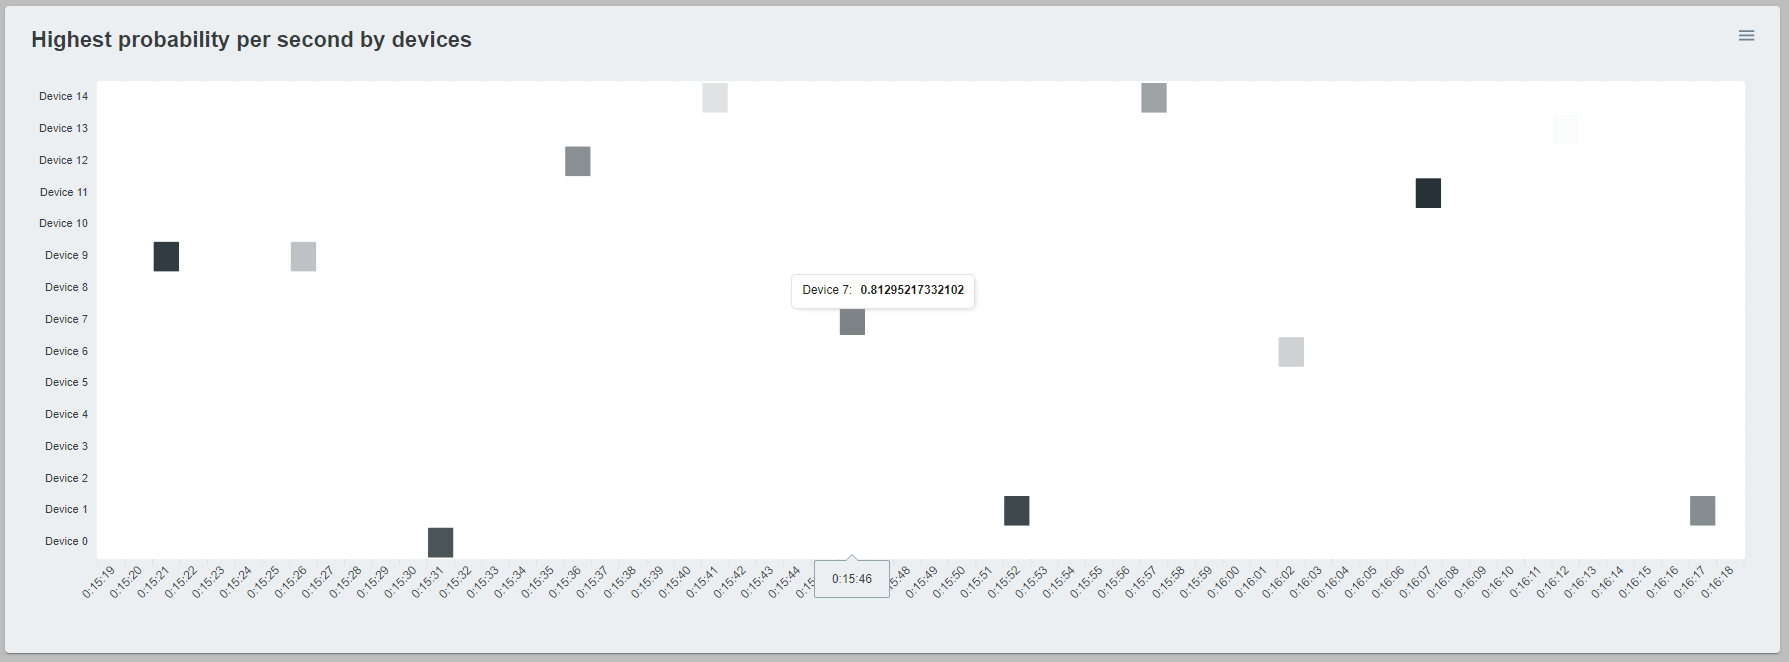
\includegraphics[width=150mm, keepaspectratio]{figures/second-heatmap.png}
    \caption{Másodperc alapú hőtérképes diagramm}
    \label{fig:dashboard-heatmap-second}
\end{figure}
\begin{figure}[!ht]
    \centering
    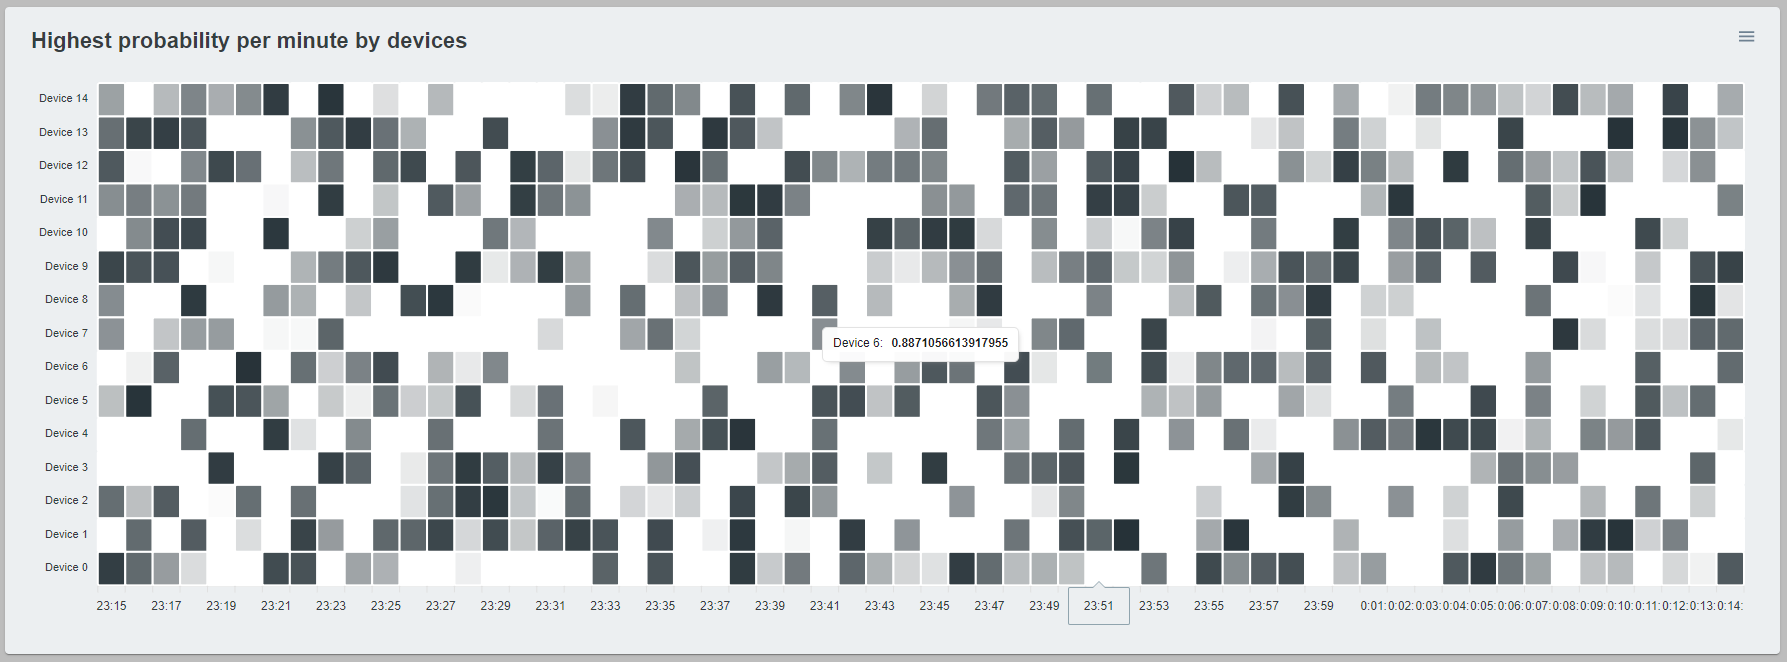
\includegraphics[width=150mm, keepaspectratio]{figures/minute-heatmap.png}
    \caption{Perc alapú hőtérképes diagramm}
    \label{fig:dashboard-heatmap-minute}
\end{figure}

A függőleges tengelyen a rendszer eszközei vannak dinamikusan megjelenítve.
A vízszintes tengelyen pedig az említett időtartományok.
A diagrammokon látható négyzetek a valószínűség nagyságától függően sötétebbek vagy világosabbak.
\newpage
%----------------------------------------------------------------------------
\subsubsection{Riasztás számláló}
%----------------------------------------------------------------------------
Ez egy egyszerű oszlopdiagram, mely aggregálja az egyes eszközök által küldött hangüzeneteket 0.5 valószínűség felett a \ref{fig:dashboard-devices-column}-es ábrán látható módon.
Segítségével megvizsgálható, hogy mely eszközök riasztanak a legtöbbet a legnagyobb valószínűséggel.
\begin{figure}[!ht]
    \centering
    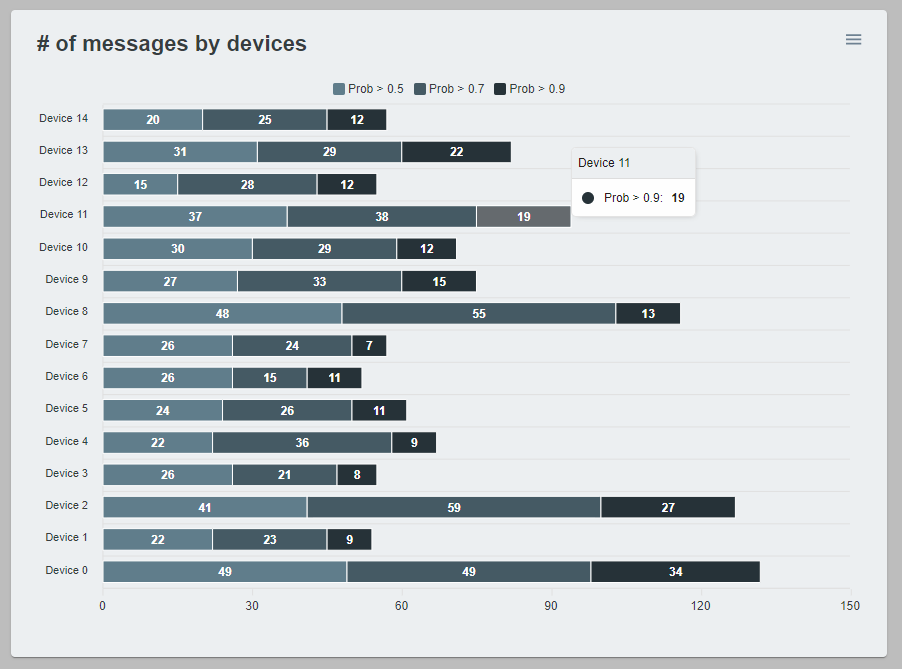
\includegraphics[width=150mm, keepaspectratio]{figures/dashboard-column-devices.png}
    \caption{Eszközönkénti riasztásokat számláló diagramm}
    \label{fig:dashboard-devices-column}
\end{figure}

Az egyes oszlopok három részre vannak bontva az üzenetek öt tized, hét tized és kilenc tized fölötti valószínűsége szerint. 
\newpage
%----------------------------------------------------------------------------
\subsubsection{Üzenetek gyakorisága}
%----------------------------------------------------------------------------
Az oldalon található utolsó diagramm egy vonal diagammn, melynek célja, hogy ábrázolja a rendszer által küldött üzenetek számát másodpercenként.
A \ref{fig:dashboard-messages-line}-es ábrán látható a komponens.
A vízszintes tengelyen a legelső érték az alkalmazás által először észlelt üzenet időpontja.
Az utolsó érték a legutoljára észlelt időpontja.
A függőleges tengelyen az adott másodpercben érkező üzenetek száma van ábrázolva.
Az előzőekkel ellentétben itt az adatok nincsennek szűrve a hangüzenet valószínűsége alapján,
tehát a rendszer által küldött összes üzenet látható.
\begin{figure}[!ht]
    \centering
    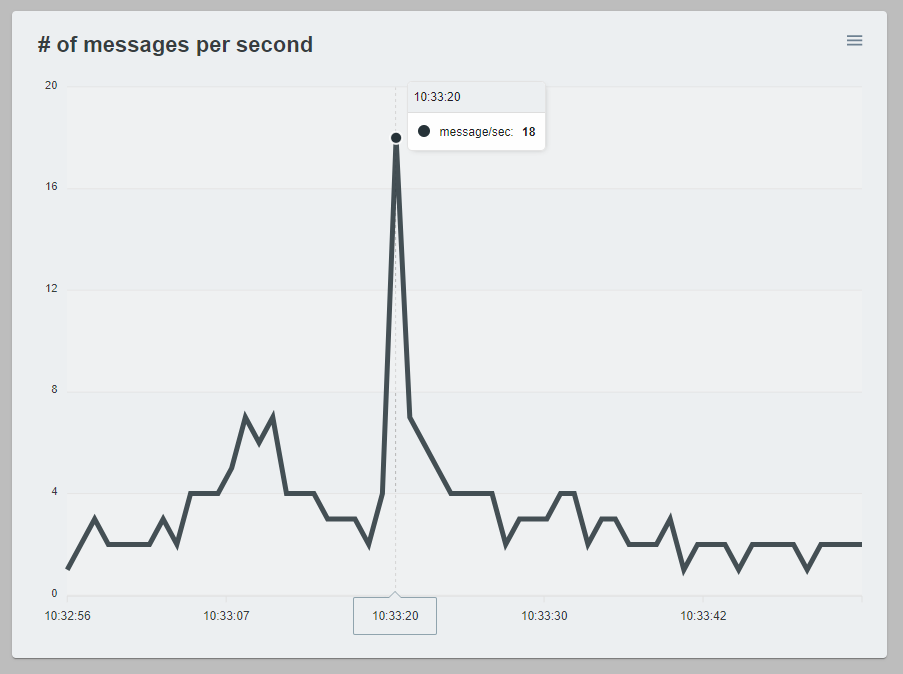
\includegraphics[width=150mm, keepaspectratio]{figures/dashboard-line-messages.png}
    \caption{A másodpercenként érkező üzenetek számát ábrázoló diagram.}
    \label{fig:dashboard-messages-line}
\end{figure}
\newpage
%----------------------------------------------------------------------------
\subsection{Devices}
%----------------------------------------------------------------------------
Ez az oldal lehetővé teszi a felhasználók számára az eszközök állapotának áttekintését, \verb+Admin+ felhasználók számára azok menedszelését is.
Az eszközök dinamikusan jelennek meg a \verb+DevicesContextProvider+ adatai alapján, melyek megjelenítésére a Material UI \verb+Accrordion+ komponensét használom.
Ennek fejlécében az eszköz neve, egyedi azonosítója és státusza található. A lenyíló részben pedig az eszköz által használt szenzorok neve, azonosítója és státusza.
\verb+Admin+ felhasználók számára a felület két fajta gombbal bővül, mellyekkel be és ki lehet kapcsolni az egyes eszközöket, szenzorokat.
Az \verb+Accordion+-ok felett található egy külön panel, mellyel egyszerre lehet kezelni az összes eszközt és azok szenzorait.
A Devices oldal felülete a \ref{fig:frontend-devices}-es ábrán,
az \verb+Admin+ felhasználók számára nyújtott plusz funkciók a \ref{fig:frontend-devices-admin}-as ábrán láthatók.
\begin{figure}[!ht]
    \centering
    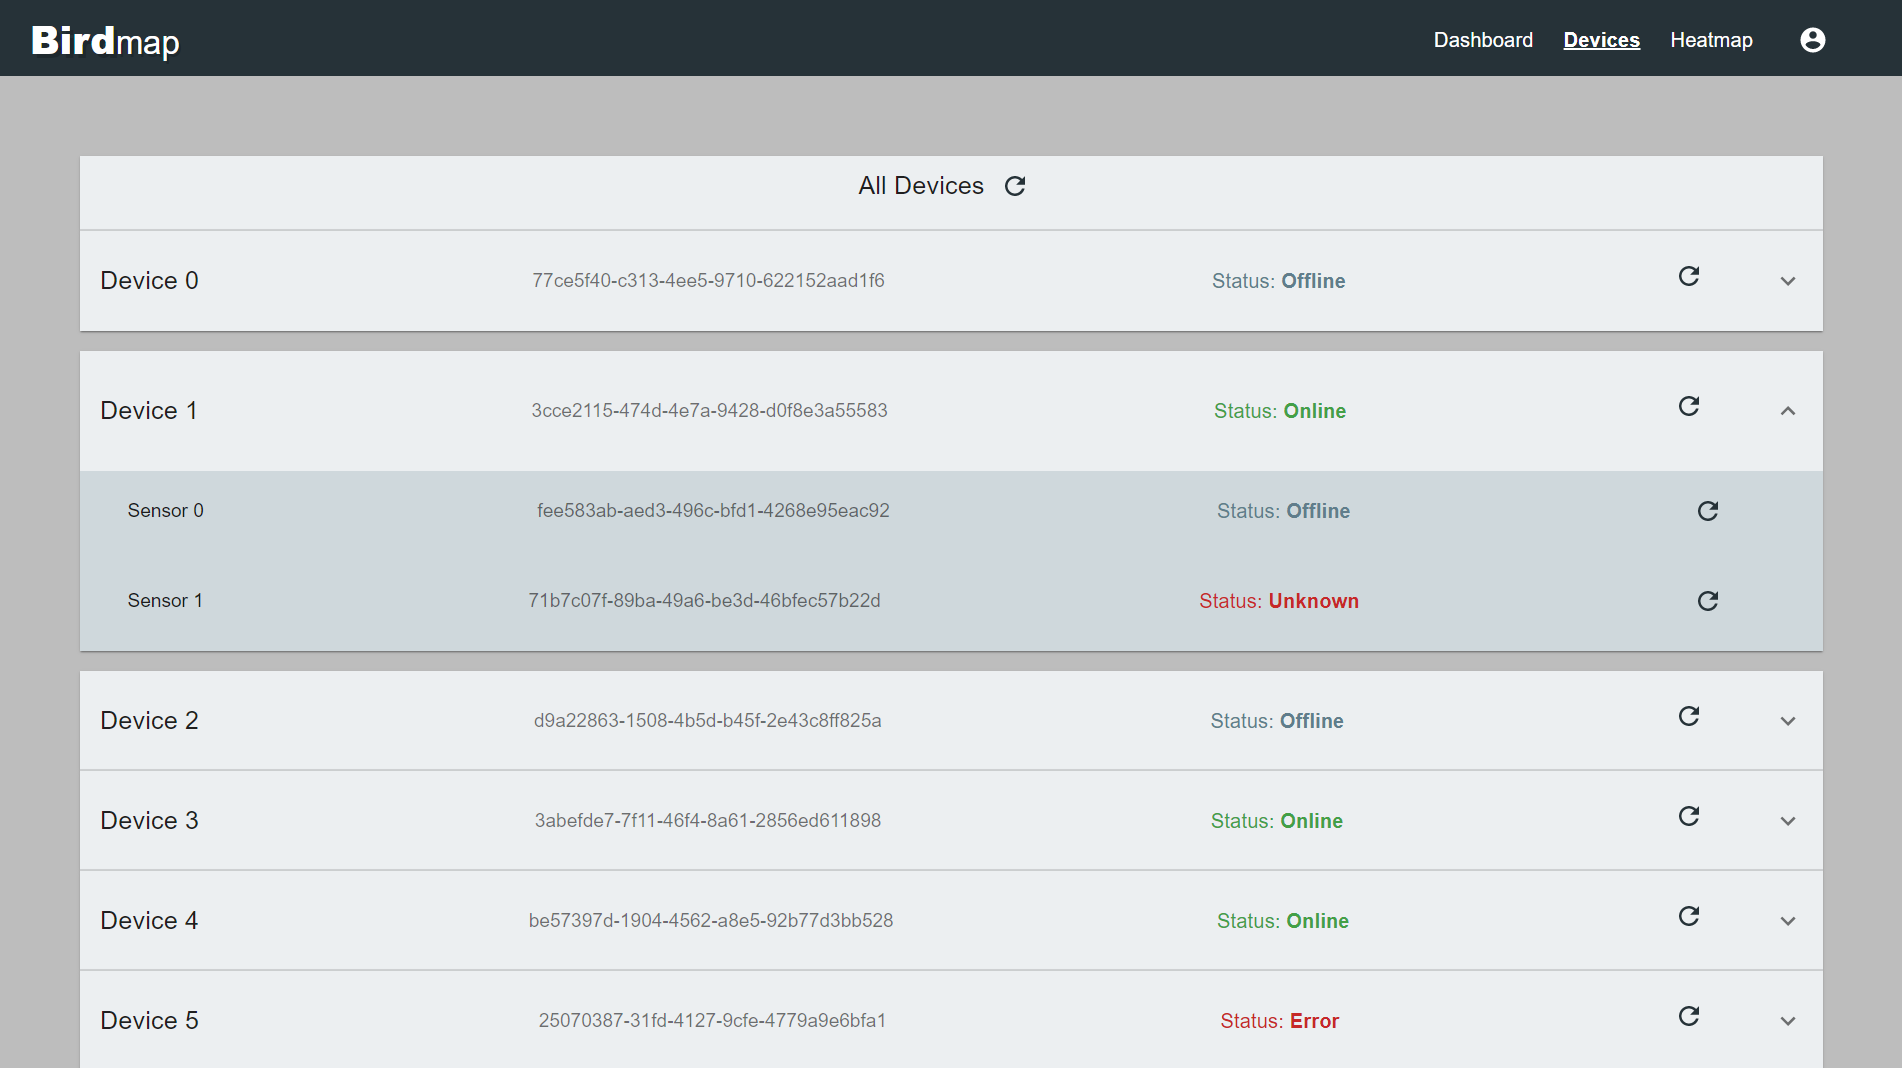
\includegraphics[width=150mm, keepaspectratio]{figures/devices.png}
    \caption{A Devices oldal felülete.}
    \label{fig:frontend-devices}
\end{figure}
\begin{figure}[!ht]
    \centering
    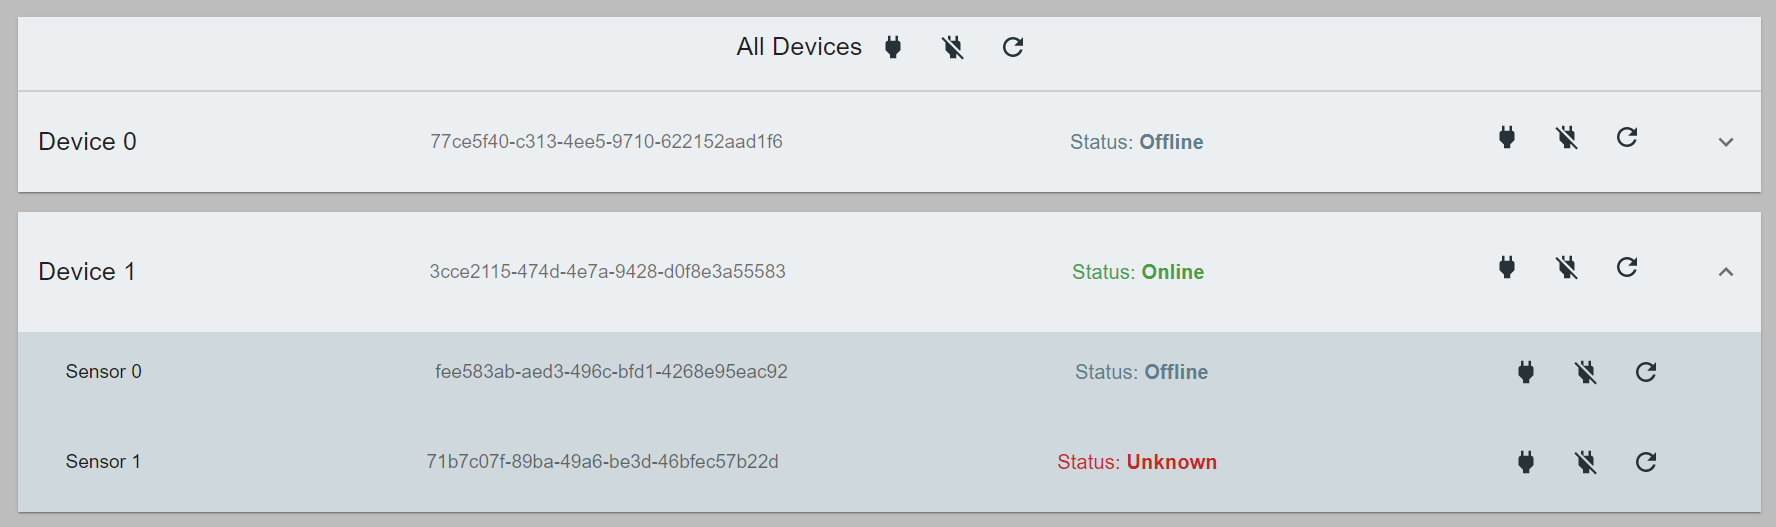
\includegraphics[width=150mm, keepaspectratio]{figures/devices-admin.png}
    \caption{Az Admin felhasználók számára elérhető plusz funkciók.}
    \label{fig:frontend-devices-admin}
\end{figure}
%----------------------------------------------------------------------------
\subsection{Heatmap}
%----------------------------------------------------------------------------
Az alkalmazással szemben az egyik legfontosabb követelmény a hőtérképes vizualizáció volt,
mely ezen az oldalon található. A Google Maps API segítségével megjelenítek egy térképet a felületen,
majd erre kerül a hőtérképes réteg. A térképre szélességi és hosszúsági körök alapján lehet rajzolni.
Ezt használva megjelenítem a rendszer összes eszközét azok koordinátái szerint.
A kék színű ikonok jelölik a bekapcsolt állapotban lévő, a sárga a kikapcsolt állapotban lévő,
a piros pedig a hibás állapotban lévő eszközöket.
Ha a felhasználó az egerét az ikonok fölé helyezi, megjelenik egy szövegdoboz, melyben az eszköz azonosítója és státusza látható. 
Az ikonra kattinta a felhasználó a Devices oldalra kerül, ahol megnyílik a kattintott eszköz \verb+Accordion+-ja.

A \verb+DevicesContext+ tartalmazza az eszközök által küldött üzenetek adatait,
melyeknek a 0.5 valószínűségtől nagyobb részhalmazát a hőtérkép által kezelhető adatokká konvertálok.
Egyrészt szükség van az előbb is említett földrajzi koordinátákra, melyeket az üzenetek eszköz azonosítója alapján határozok meg.
Másrészt szükség van egy súly értékre, mely a pont színezésének pirosságát határozza meg.
Ezt az értéket az üzenetek valószínűség értékével tettem egyenlővé.
Minnél több magasabb valószínűségű riasztás érkezik egy adott eszköztől, a körülötte lévő terület annál pirosabb lesz.

A \ref{fig:frontend-heatmap}-ös ábra mutatja a térkép működését miközben 4 eszköz is seregélyeket észelt.

\begin{figure}[!ht]
    \centering
    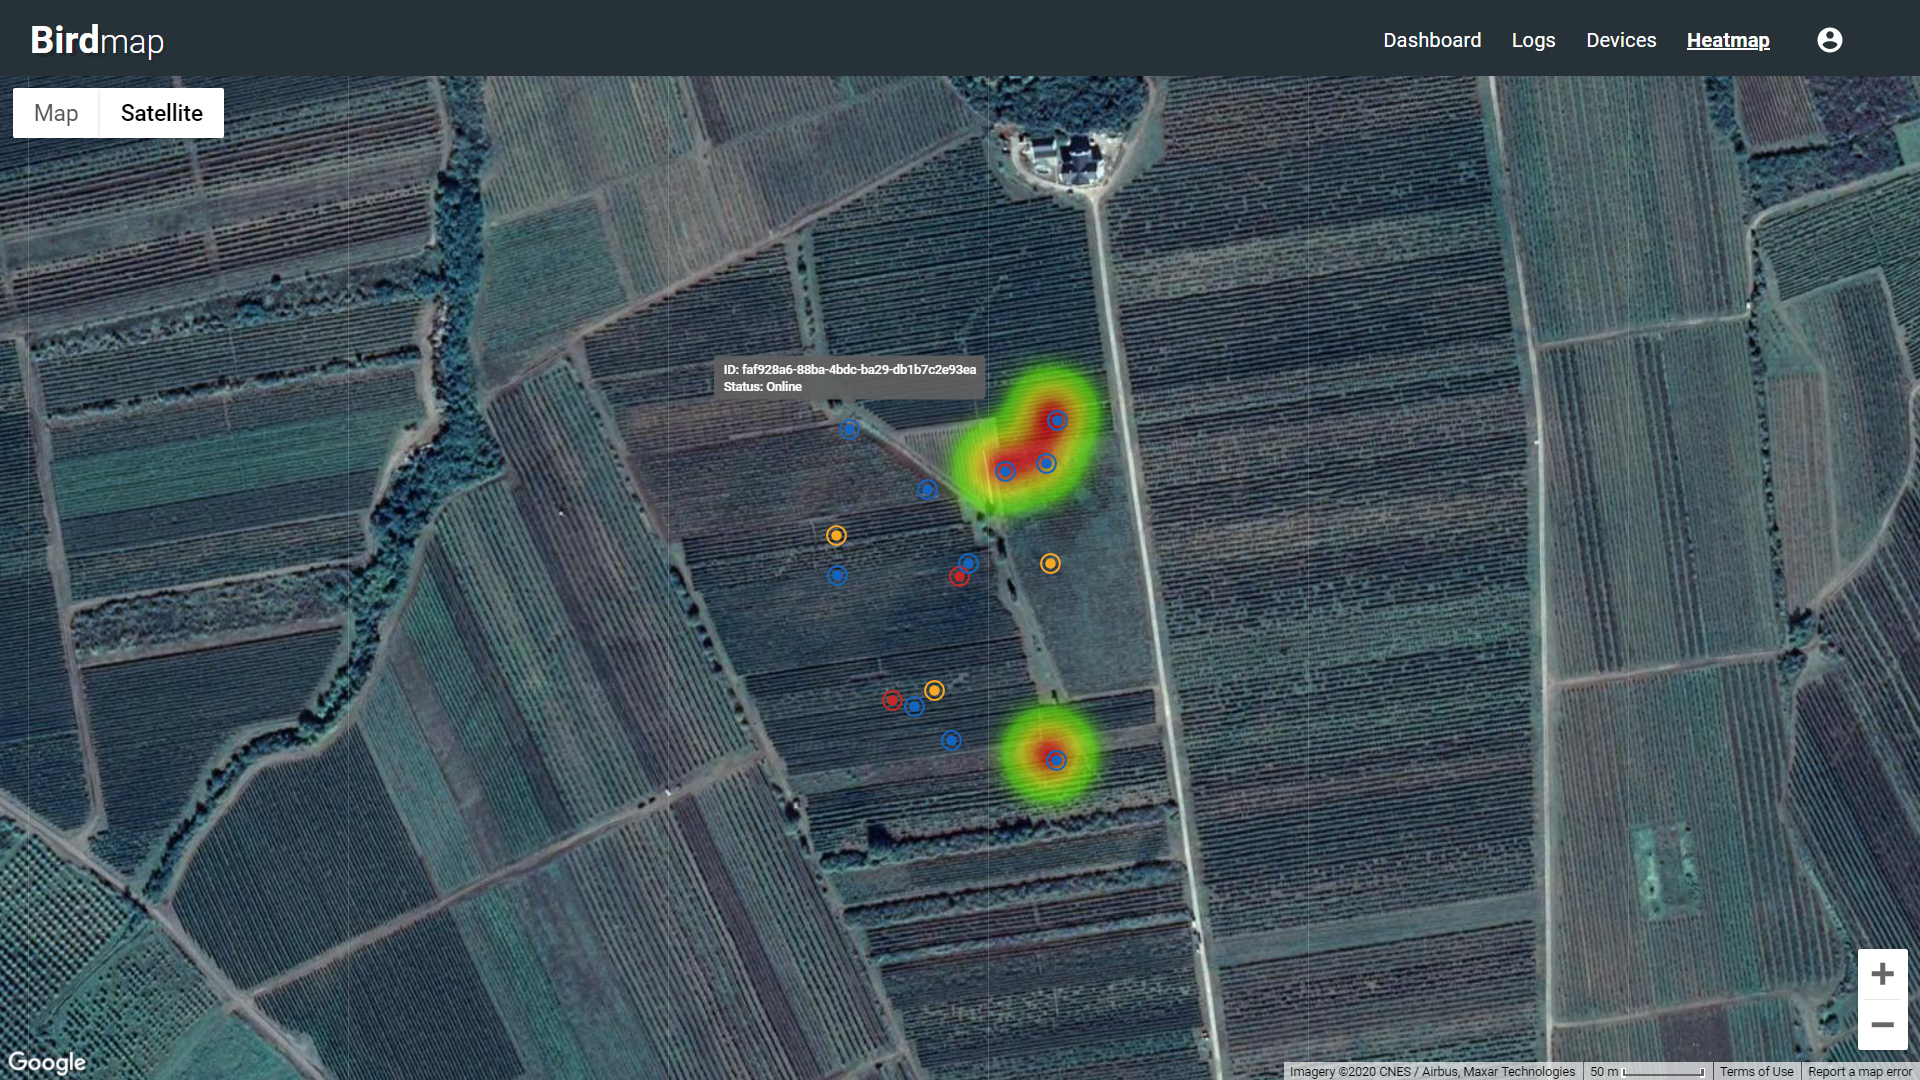
\includegraphics[width=150mm, keepaspectratio]{figures/heatmap.png}
    \caption{A Heatmap oldal felülete.}
    \label{fig:frontend-heatmap}
\end{figure}